% ---------------------------------------------------------------------------
% The rope snaps, break by break: the b quark's string of our event (the -v
% log, string 1), with the gluon kinks left out of the drawing. Each row is
% the string that is left, the end that fires and the pair that appears; the
% peeled-off hadrons accumulate on the left (from the b end) and on the right
% (from the ubar end). The last row is the full chain of sixteen with the
% vacuum pair written between every two neighbours: the quark of each pair
% went into the hadron on its right, the antiquark into the one on its left.
% ---------------------------------------------------------------------------
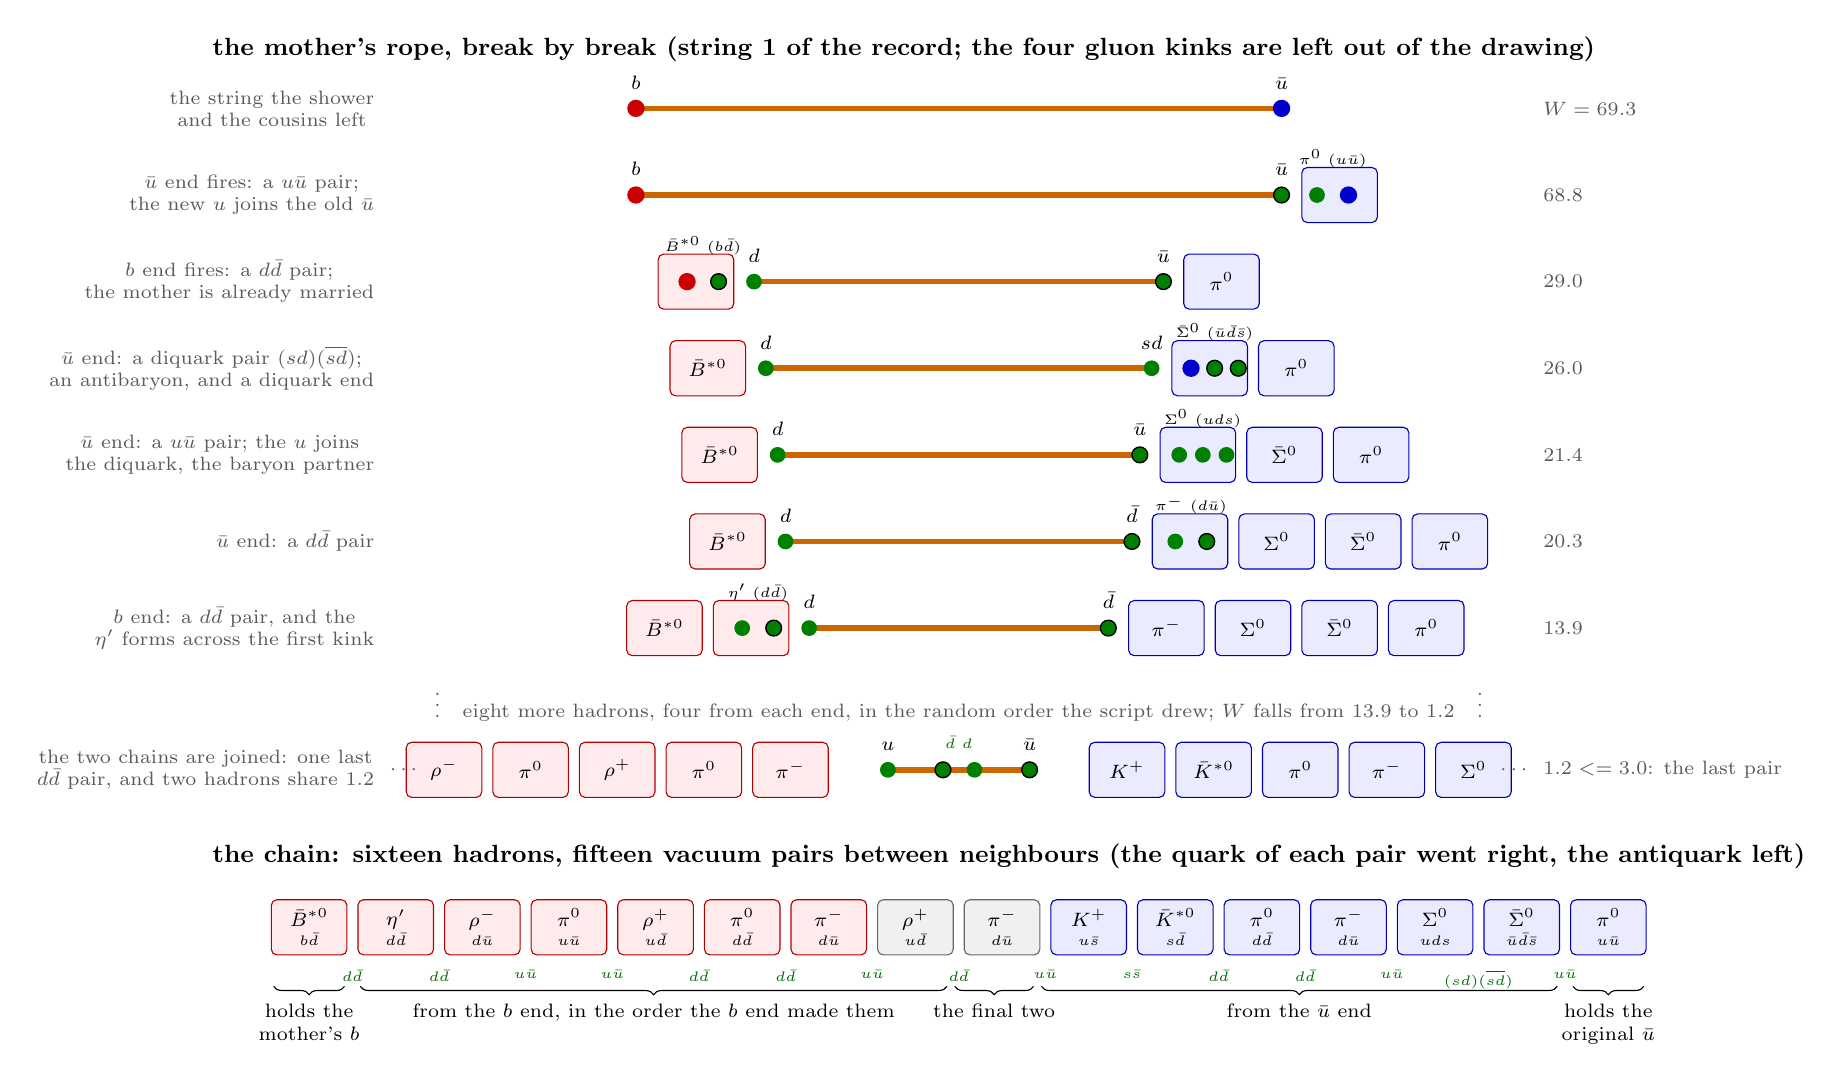
\begin{tikzpicture}[x=1cm,y=1cm,
  every node/.style={font=\footnotesize},
  q/.style={circle,inner sep=0pt,minimum size=2.2mm,fill=red!80!black},
  aq/.style={circle,inner sep=0pt,minimum size=2.2mm,fill=blue!80!black},
  nq/.style={circle,inner sep=0pt,minimum size=2.0mm,fill=green!50!black},
  naq/.style={circle,inner sep=0pt,minimum size=2.0mm,fill=green!50!black,draw=black,line width=0.5pt},
  rope/.style={orange!80!black,line width=2.0pt},
  hb/.style={rounded corners=2pt,draw=red!70!black,fill=red!8,minimum width=9.6mm,minimum height=7mm,inner sep=1pt,align=center,font=\scriptsize},
  hu/.style={rounded corners=2pt,draw=blue!70!black,fill=blue!8,minimum width=9.6mm,minimum height=7mm,inner sep=1pt,align=center,font=\scriptsize},
  hf/.style={rounded corners=2pt,draw=black!60,fill=black!6,minimum width=9.6mm,minimum height=7mm,inner sep=1pt,align=center,font=\scriptsize},
  lab/.style={font=\scriptsize,align=center},
  tiny/.style={font=\tiny,align=center},
  head/.style={font=\small\bfseries}]
% a row: \chainrow{y}{half length}{left end label}{right end label}{W text}
\def\chainrow#1#2#3#4#5{\draw[rope] (-#2,#1) -- (#2,#1);
  \node[lab,anchor=south] at (-#2,#1+0.12) {#3}; \node[lab,anchor=south] at (#2,#1+0.12) {#4};
  \node[lab,anchor=west,text=black!65] at (7.3,#1) {#5};}
% ---- row 0: the string as the shower left it
\node[head,anchor=west] at (-9.6,8.15) {the mother's rope, break by break (string~1 of the record; the four gluon kinks are left out of the drawing)};
\chainrow{7.4}{4.1}{$b$}{$\bar u$}{$W=69.3\GeV$}
\node[q] at (-4.1,7.4) {}; \node[aq] at (4.1,7.4) {};
\node[lab,anchor=east,text=black!65] at (-7.3,7.4) {the string the shower\\ and the cousins left};
% ---- row 1: ubar end, pair u ubar -> pi0
\chainrow{6.3}{4.1}{$b$}{$\bar u$}{$68.8$}
\node[q] at (-4.1,6.3) {}; \node[naq] at (4.1,6.3) {};
\node[hu,anchor=west] at (4.35,6.3) {\phantom{$\pi^0$}}; \node[nq] at (4.55,6.3) {}; \node[aq] at (4.95,6.3) {};
\node[tiny,anchor=south] at (4.75,6.52) {$\pi^0\ (u\bar u)$};
\node[lab,anchor=east,text=black!65] at (-7.3,6.3) {$\bar u$ end fires: a $u\bar u$ pair;\\ the new $u$ joins the old $\bar u$};
% ---- row 2: b end, pair d dbar -> B*bar0
\chainrow{5.2}{2.6}{$d$}{$\bar u$}{$29.0$}
\node[nq] at (-2.6,5.2) {}; \node[naq] at (2.6,5.2) {};
\node[hb,anchor=east] at (-2.85,5.2) {\phantom{$\bar B^{*0}$}}; \node[q] at (-3.45,5.2) {}; \node[naq] at (-3.05,5.2) {};
\node[tiny,anchor=south] at (-3.25,5.42) {$\bar B^{*0}\ (b\bar d)$};
\node[hu,anchor=west] at (2.85,5.2) {$\pi^0$};
\node[lab,anchor=east,text=black!65] at (-7.3,5.2) {$b$ end fires: a $d\bar d$ pair;\\ the mother is already married};
% ---- row 3: ubar end, diquark pair -> Sigmabar0
\chainrow{4.1}{2.45}{$d$}{$sd$}{$26.0$}
\node[nq] at (-2.45,4.1) {}; \node[nq] at (2.45,4.1) {};
\node[hb,anchor=east] at (-2.7,4.1) {$\bar B^{*0}$};
\node[hu,anchor=west] at (2.7,4.1) {\phantom{$\bar\Sigma^0$}}; \node[aq] at (2.95,4.1) {}; \node[naq] at (3.25,4.1) {}; \node[naq] at (3.55,4.1) {};
\node[tiny,anchor=south] at (3.25,4.32) {$\bar\Sigma^0\ (\bar u\bar d\bar s)$};
\node[hu,anchor=west] at (3.8,4.1) {$\pi^0$};
\node[lab,anchor=east,text=black!65] at (-7.3,4.1) {$\bar u$ end: a diquark pair $(sd)(\overline{sd})$;\\ an antibaryon, and a diquark end};
% ---- row 4: ubar end, pair u ubar -> Sigma0
\chainrow{3.0}{2.3}{$d$}{$\bar u$}{$21.4$}
\node[nq] at (-2.3,3.0) {}; \node[naq] at (2.3,3.0) {};
\node[hb,anchor=east] at (-2.55,3.0) {$\bar B^{*0}$};
\node[hu,anchor=west] at (2.55,3.0) {\phantom{$\Sigma^0$}}; \node[nq] at (2.8,3.0) {}; \node[nq] at (3.1,3.0) {}; \node[nq] at (3.4,3.0) {};
\node[tiny,anchor=south] at (3.1,3.22) {$\Sigma^0\ (uds)$};
\node[hu,anchor=west] at (3.65,3.0) {$\bar\Sigma^0$}; \node[hu,anchor=west] at (4.75,3.0) {$\pi^0$};
\node[lab,anchor=east,text=black!65] at (-7.3,3.0) {$\bar u$ end: a $u\bar u$ pair; the $u$ joins\\ the diquark, the baryon partner};
% ---- row 5: ubar end, pair d dbar -> pi-
\chainrow{1.9}{2.2}{$d$}{$\bar d$}{$20.3$}
\node[nq] at (-2.2,1.9) {}; \node[naq] at (2.2,1.9) {};
\node[hb,anchor=east] at (-2.45,1.9) {$\bar B^{*0}$};
\node[hu,anchor=west] at (2.45,1.9) {\phantom{$\pi^-$}}; \node[nq] at (2.75,1.9) {}; \node[naq] at (3.15,1.9) {};
\node[tiny,anchor=south] at (2.95,2.12) {$\pi^-\ (d\bar u)$};
\node[hu,anchor=west] at (3.55,1.9) {$\Sigma^0$}; \node[hu,anchor=west] at (4.65,1.9) {$\bar\Sigma^0$}; \node[hu,anchor=west] at (5.75,1.9) {$\pi^0$};
\node[lab,anchor=east,text=black!65] at (-7.3,1.9) {$\bar u$ end: a $d\bar d$ pair};
% ---- row 6: b end, pair d dbar -> eta'
\chainrow{0.8}{1.9}{$d$}{$\bar d$}{$13.9$}
\node[nq] at (-1.9,0.8) {}; \node[naq] at (1.9,0.8) {};
\node[hb,anchor=east] at (-2.15,0.8) {\phantom{$\eta'$}}; \node[nq] at (-2.75,0.8) {}; \node[naq] at (-2.35,0.8) {};
\node[tiny,anchor=south] at (-2.55,1.02) {$\eta'\ (d\bar d)$};
\node[hb,anchor=east] at (-3.25,0.8) {$\bar B^{*0}$};
\node[hu,anchor=west] at (2.15,0.8) {$\pi^-$}; \node[hu,anchor=west] at (3.25,0.8) {$\Sigma^0$}; \node[hu,anchor=west] at (4.35,0.8) {$\bar\Sigma^0$}; \node[hu,anchor=west] at (5.45,0.8) {$\pi^0$};
\node[lab,anchor=east,text=black!65] at (-7.3,0.8) {$b$ end: a $d\bar d$ pair, and the\\ $\eta'$ forms across the first kink};
% ---- row 7: dots
\node[lab,text=black!65] at (0,-0.1) {$\vdots$\quad eight more hadrons, four from each end, in the random order the script drew; $W$ falls from $13.9$ to $1.2\GeV$\quad$\vdots$};
% ---- row 8: the final two
\chainrow{-1.0}{0.9}{$u$}{$\bar u$}{$1.2<\Wmin=3.0\GeV$: the last pair}
\node[nq] at (-0.9,-1.0) {}; \node[naq] at (0.9,-1.0) {};
\node[naq] at (-0.2,-1.0) {}; \node[nq] at (0.2,-1.0) {}; \node[tiny,text=green!40!black,anchor=south] at (0,-0.85) {$\bar d\ d$};
\node[lab,anchor=east,text=black!65] at (-7.3,-1.0) {the two chains are joined: one last\\ $d\bar d$ pair, and two hadrons share $1.2\GeV$};
\foreach \x/\n in {-1.65/{$\pi^-$},-2.75/{$\pi^0$},-3.85/{$\rho^+$},-4.95/{$\pi^0$},-6.05/{$\rho^-$}} {\node[hb,anchor=east] at (\x,-1.0) {\n};}
\foreach \x/\n in {1.65/{$K^+$},2.75/{$\bar K^{*0}$},3.85/{$\pi^0$},4.95/{$\pi^-$},6.05/{$\Sigma^0$}} {\node[hu,anchor=west] at (\x,-1.0) {\n};}
\node[lab,text=black!65] at (-7.05,-1.0) {$\cdots$}; \node[lab,text=black!65] at (7.05,-1.0) {$\cdots$};
% ---- row 9: the chain of sixteen with the pairs between neighbours
\node[head,anchor=west] at (-9.6,-2.1) {the chain: sixteen hadrons, fifteen vacuum pairs between neighbours (the quark of each pair went right, the antiquark left)};
\def\chainbox#1#2#3#4{\node[#4] at (#1*1.1-8.25,-3.0) {#2\\[-1pt] {\tiny #3}};}
\chainbox{0}{$\bar B^{*0}$}{$b\bar d$}{hb}
\chainbox{1}{$\eta'$}{$d\bar d$}{hb}
\chainbox{2}{$\rho^-$}{$d\bar u$}{hb}
\chainbox{3}{$\pi^0$}{$u\bar u$}{hb}
\chainbox{4}{$\rho^+$}{$u\bar d$}{hb}
\chainbox{5}{$\pi^0$}{$d\bar d$}{hb}
\chainbox{6}{$\pi^-$}{$d\bar u$}{hb}
\chainbox{7}{$\rho^+$}{$u\bar d$}{hf}
\chainbox{8}{$\pi^-$}{$d\bar u$}{hf}
\chainbox{9}{$K^+$}{$u\bar s$}{hu}
\chainbox{10}{$\bar K^{*0}$}{$s\bar d$}{hu}
\chainbox{11}{$\pi^0$}{$d\bar d$}{hu}
\chainbox{12}{$\pi^-$}{$d\bar u$}{hu}
\chainbox{13}{$\Sigma^0$}{$uds$}{hu}
\chainbox{14}{$\bar\Sigma^0$}{$\bar u\bar d\bar s$}{hu}
\chainbox{15}{$\pi^0$}{$u\bar u$}{hu}
\foreach \i/\p in {0/{$d\bar d$},1/{$d\bar d$},2/{$u\bar u$},3/{$u\bar u$},4/{$d\bar d$},5/{$d\bar d$},6/{$u\bar u$},7/{$d\bar d$},8/{$u\bar u$},9/{$s\bar s$},10/{$d\bar d$},11/{$d\bar d$},12/{$u\bar u$},13/{$(sd)(\overline{sd})$},14/{$u\bar u$}} {
  \node[tiny,text=green!40!black,anchor=north] at (\i*1.1-7.7,-3.42) {\p};}
\draw[decorate,decoration={brace,mirror,amplitude=3pt}] (-8.7,-3.75) -- (-7.8,-3.75) node[midway,below=3pt,lab] {holds the\\ mother's $b$};
\draw[decorate,decoration={brace,mirror,amplitude=3pt}] (7.8,-3.75) -- (8.7,-3.75) node[midway,below=3pt,lab] {holds the\\ original $\bar u$};
\draw[decorate,decoration={brace,mirror,amplitude=3pt}] (-7.6,-3.75) -- (-0.15,-3.75) node[midway,below=3pt,lab] {from the $b$ end, in the order the $b$ end made them};
\draw[decorate,decoration={brace,mirror,amplitude=3pt}] (-0.05,-3.75) -- (0.95,-3.75) node[midway,below=3pt,lab] {the final two};
\draw[decorate,decoration={brace,mirror,amplitude=3pt}] (1.05,-3.75) -- (7.6,-3.75) node[midway,below=3pt,lab] {from the $\bar u$ end};
\end{tikzpicture}
